\documentclass{article}

\usepackage{graphicx}
\usepackage{subfigure}
\usepackage[hypcap]{caption}
\usepackage{listings}
\usepackage{float}
\floatstyle{plaintop}
\restylefloat{table}
\usepackage[hidelinks]{hyperref}

\title{Experimental Design and Data Analysis: \\ \large{Calcium, inorganic phosphorus and alkaline phosphatase levels\\ in elderly patients}}
\author{Andrew Bedard(2566978) \& Simone van Gompel(2567525) \\ Group 19}

\begin{document}

  \maketitle

  \section{Introduction}
    In this paper the process of analysing a certain dataset is laid out.
    The dataset used is calcium.dat, which can be found at \url{http://www.amstat.org/publications/jse/jse_data_archive.htm}.
    This dataset is used for this project, because it has a good number of entries and enough features to be able to do data analysis on.
    In the rest of this paper the experiment is explained, the data is analyzed, the results are shown and the process is discussed.
    In the appendix the used R code is shown.

  \section{The Experiment}
    The experiment was set up with the goal to see if age and sex has an influence on certain concentrations in the body.
    The concentrations that were measured are:
    \begin{itemize}
      \item Alkaline Phosphatase International Units/Liter (Alksphos)
      \item Calcium mmol/L (Cammol)
      \item Inorganic Phosphorus mmol/L (Phosmmol)
    \end{itemize}
    There are 6 different labs from which the data is extracted.
    Next to these features, the sex, age, agegroup and patient observation number are recorded.
    In the calcium.dat the original data is stored with errors, in calciumgood.dat the data is already cleaned up.
    In this project only the calcium.dat data is used to explain how the cleaning up of the data is done.
    The research question we want to answer is: What influence does age have on the given concentrations in the body?

  \section{Data Analysis}
    \subsection{Preparation}
      The data needed to be prepared to be able to read it in R.
      This preparation exists of replacing the empty fields by an underscore, with this the data can be read in R.
      First off a pairs plot was made of the data to be able to see how the data relates to each other.
      In Fig\ref{fig:OrgPairs} the foremost problem is clear, the outliers in the data are big and not logical.
      Furthermore has Lab more than 6 categories, these problems can be explained by human error.
      And lastly the lab 3 has strange measurements with the cammol, this might be because of confusion of the measurement unit.
      The following values were changed:
      \begin{itemize}
        \item Removed Ages over 110
        \item Removed Sex which is not in the category 1 or 2
        \item Removed Lab categories which are over 6
        \item Removed Phosmmol over 2 and under 0.2
        \item Divided Cammol of Lab 3 by 10 (this is visually tested by using a pairs plot)
        \item Removed Cammol over 3 and under 1.9
        \item Removed Alksphos over 150 and under 20
      \end{itemize}
      After removal the same plot is made, see: Fig\ref{fig:UpdPairs}.
      Here you can see the correlations between the features better than in Fig\ref{fig:OrgPairs}.
      \begin{figure}
          \centering
          \subfigure[Original Data]
          {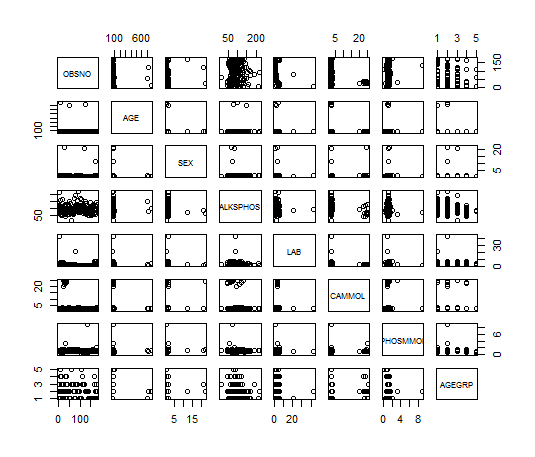
\includegraphics[scale=0.3]{../results/FirstPairs.png}\label{fig:OrgPairs}}
          \subfigure[Updated Data]
          {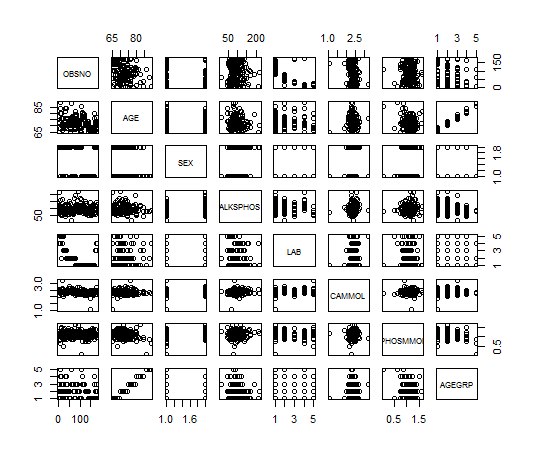
\includegraphics[scale=0.3]{../results/SecondPairs.png}\label{fig:UpdPairs}}
          \caption{Pairsplot of the data}
          \label{fig:Pairs}
      \end{figure}

    \subsection{Analysis}
      The feature that needs to be analyzed is age, this can be done by either using the feature age or the feature age group.
      The age group exists of 5 levels and is thus categorical.
      The different age groups are: 1=65-69, 2=70-74, 3=75-79, 4=80-84, 5=85-89 Years.
      In Fig\ref{fig:BoxAgegrp} the relation between the different concentrations and the age groups are visually represented.

      \begin{figure}[H]
          \centering
          \subfigure[Alksphos]{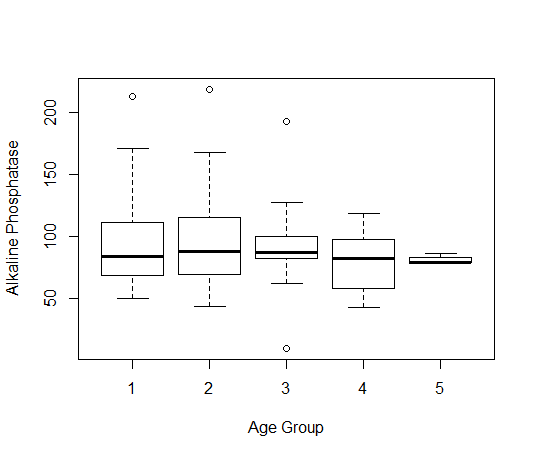
\includegraphics[scale=0.2]{../results/BoxAlksphosAgegrp.png}}
          \subfigure[Cammol]{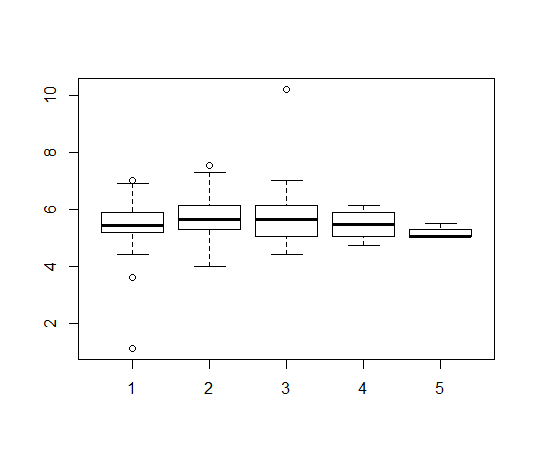
\includegraphics[scale=0.2]{../results/BoxCammolAgegrp.png}}
          \subfigure[Phosmmol]{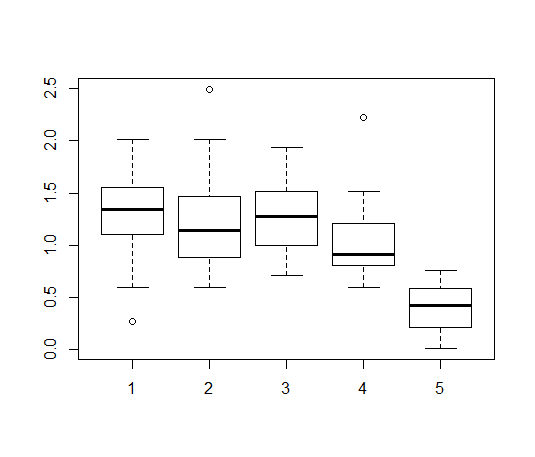
\includegraphics[scale=0.2]{../results/BoxPhosmmolAgegrp.png}}
          \caption{Boxplots of the concentrations with the age groups}
          \label{fig:BoxAgegrp}
      \end{figure}

	Analysing whether the data in CAMMOL, ALKSPHOS and PHOSMMOL is normal:
	
	\begin{figure}[H]
		\centering
		{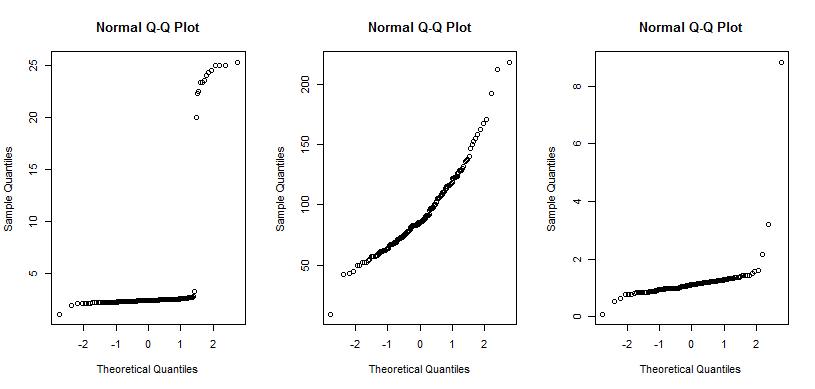
\includegraphics[scale=0.3]{../results/dat1_qq.png}}
		\caption{QQ plot of raw data}
		\label{fig:qq1}
	\end{figure}
	
	Obviously these are not normal, most likely due to outliers. After removing outliers we obtain:
	
	\begin{figure}[H]
		\centering
		{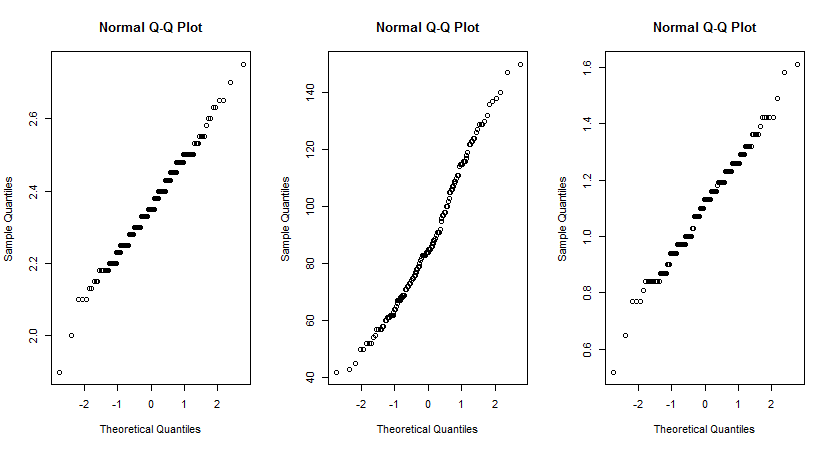
\includegraphics[scale=0.3]{../results/dat2_qq.png}}
		\caption{QQ plot after removing outliers}
		\label{fig:qq2}
	\end{figure}
	
	Clearly these are more likely normal, even though we do have a step type pattern, likely due to rounding.
	
      As see in Fig\ref{fig:BoxAgegrp} there is some difference between the different age groups with all of the concentrations.
      But with Alksphos the difference only seems to be in the variety of the values, the same holds for Cammol.
      For Phosmmol there does seems to be a difference in the age groups, the median drops with the older ages.
      The difference in the first two concentrations is because of the number of people in the different age groups, see Table\ref{table:Agegrp}.
      This shows that there are only three patients in the last age group and not too much in the group before that.
      This explains that the variety seems to lower with the higher age groups.
      
      \begin{table}[H]
        \begin{center}
          \scriptsize
          \begin{tabular}{|l|lllll|}
          \hline
          Groups&1&2&3&4&5\\
          \hline
          Patients&56&70&38&10&3\\
          \hline
          \end{tabular}
        \end{center}
        \caption{The number of patients per age group}
        \label{table:Agegrp}
      \end{table}

      To see if sex, lab and age have an influence on the concentrations, the interaction plots in Fig\ref{fig:IntLabSex} and Fig\ref{fig:IntAgeSex} are made.
      This shows that all three features have an influence on the measured concentrations.
      The age has an influence over the concentrations, which is good for the research question. 
      But the lab and sex also influence the outcome, which means that these need to be taken into account with modeling the data.

      \begin{figure}[H]
          \centering
          \subfigure[Alksphos]{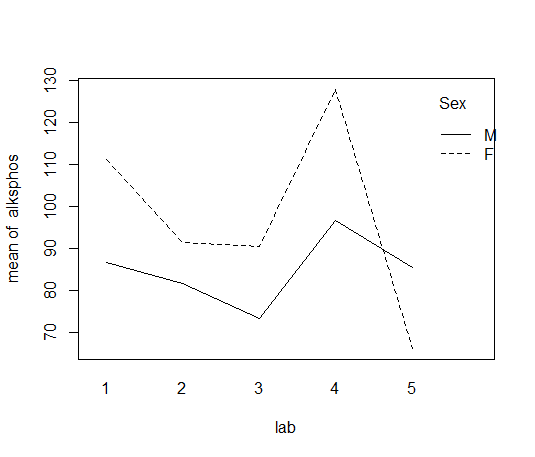
\includegraphics[scale=0.2]{../results/AlkLabSex.png}}
          \subfigure[Cammol]{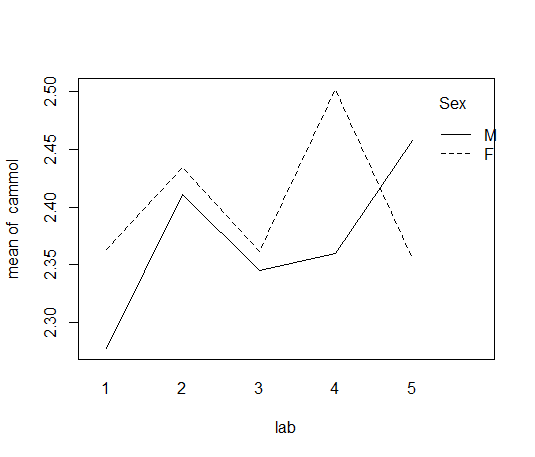
\includegraphics[scale=0.2]{../results/CamLabSex.png}}
          \subfigure[Phosmmol]{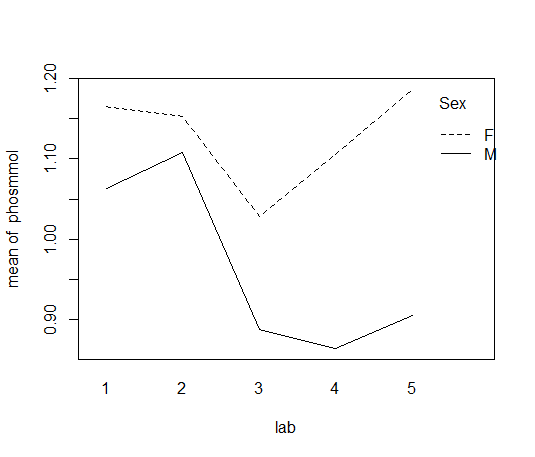
\includegraphics[scale=0.2]{../results/PhosLabSex.png}}
          \caption{Interaction plots of the sex and labs of the different concentrations}
          \label{fig:IntLabSex}
      \end{figure}
      \begin{figure}[H]
          \centering
          \subfigure[Alksphos]{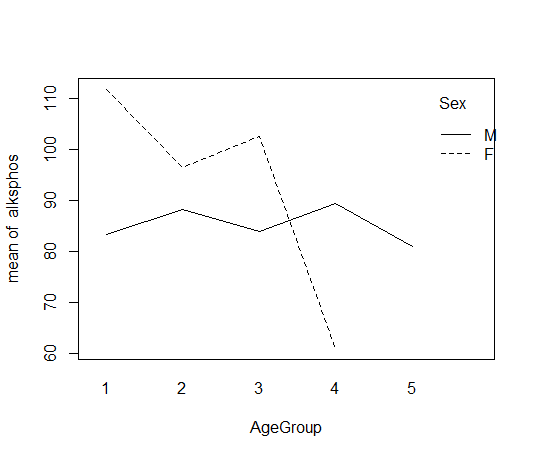
\includegraphics[scale=0.2]{../results/AlkAgeSex.png}}
          \subfigure[Cammol]{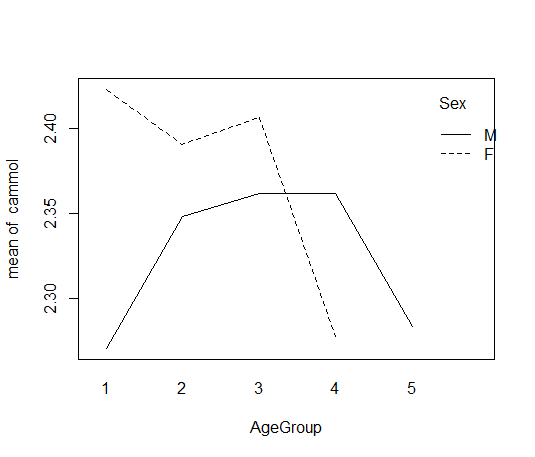
\includegraphics[scale=0.2]{../results/CamAgeSex.png}}
          \subfigure[Phosmmol]{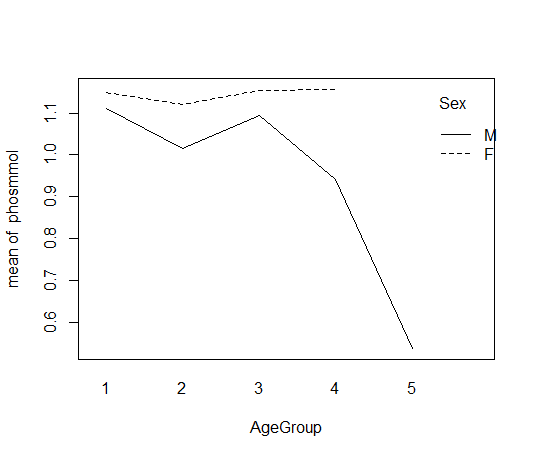
\includegraphics[scale=0.2]{../results/PhosAgeSex.png}}
          \caption{Interaction plots of the sex and age groups of the different concentrations}
          \label{fig:IntAgeSex}
      \end{figure}
      
          \begin{table}[H]
    \begin{center}
    \scriptsize
    \begin{tabular}{|ll|}
        \hline
        Variable & \textit{p} \\
        \hline 
        \hline
        CAMMOL\textasciitilde SEX & 0.001539 \\
        CAMMOL\textasciitilde LAB & 1.433e-05 \\
        CAMMOL\textasciitilde AGEGRP & 0.5451 \\
        \hline
        \hline 
        ALKSPHOS\textasciitilde SEX & 0.007631 \\
        ALKSPHOS\textasciitilde LAB & 0.001325 \\
        ALKSPHOS\textasciitilde AGEGRP & 0.6927 \\
        \hline
        \hline 
        PHOSMMOL\textasciitilde SEX & 0.007711 \\
        PHOSMMOL\textasciitilde LAB & 0.159 \\
        PHOSMMOL\textasciitilde AGEGRP & 0.006144 \\
        \hline
    \end{tabular}
    \caption{Kruskal-Wallis rank sum test}
    \label{table:krusk}
    \end{center}
    \end{table}

    \begin{table}
    \begin{center}
    \scriptsize
    \begin{tabular}{|l|l|l|l|}
      \hline
      &$SEX * LAB$&$SEX * AGEGRP$&$LAB*AGEGRP$\\
      \hline
      $Var1$       & 0.00012 & 0.0003835 & 1.491e-05\\
      $Var2$       & 0.00015 & 0.9361766 & 0.4083\\
      $Var1:Var2$  & 0.51331 & 0.1214165 & 0.6595\\
      \hline
    \end{tabular}
    \caption{Anova, response variable: Cammol}
    \label{table:AnCammol}
    \end{center}
    \end{table}

    \begin{table}
    \begin{center}
    \scriptsize
    \begin{tabular}{|l|l|l|l|}
      \hline
      &$SEX * LAB$&$SEX * AGEGRP$&$LAB*AGEGRP$\\
      \hline
      $Var1$       & 0.05781 & 0.07838 & 0.03025\\
      $Var2$       & 0.01471 & 0.63871 & 0.72707\\
      $Var1:Var2$  & 0.53010 & 0.08933 & 0.58935\\
      \hline
    \end{tabular}
    \caption{Anova, response variable: Alsphos}
    \label{table:AnAlsphos}
    \end{center}
    \end{table}

    \begin{table}
    \begin{center}
    \scriptsize
    \begin{tabular}{|l|l|l|l|}
      \hline
      &$SEX * LAB$&$SEX * AGEGRP$&$LAB*AGEGRP$\\
      \hline
      $Var1$       & 0.002991 & 0.003218 & 0.18946\\
      $Var2$       & 0.006101 & 0.007732 & 0.02311\\
      $Var1:Var2$  & 0.207392 & 0.402506 & 0.16321\\
      \hline
    \end{tabular}
    \caption{Anova, response variable: Phosmmol}
    \label{table:AnPhosmmol}
    \end{center}
    \end{table}
    
    \subsection{Modeling}
      Modeling the data can be done in several ways.
      The first one tried is a step down linear regression approach for each of the concentrations.
      For Alksphos it follows the following steps:
      \begin{itemize}
        \scriptsize{\item $ALKSPHOS \sim AGE + SEX + LAB + AGEGRP$}
        \scriptsize{\item $ALKSPHOS \sim AGE + SEX + LAB$}
        \scriptsize{\item $ALKSPHOS \sim SEX + LAB$}
        \scriptsize{\item $ALKSPHOS = 88.96 + 17.91*SEX2 - 11.69*LAB2 - 16.25*LAB3 + 18.03*LAB4 - 30.20*LAB5$}
      \end{itemize}
      For Cammol it follows the following steps:
      \begin{itemize}
        \scriptsize{\item $CAMMOL \sim AGE + SEX + LAB + AGEGRP$}
        \scriptsize{\item $CAMMOL \sim AGE + SEX + LAB$}
        \scriptsize{\item $CAMMOL \sim SEX + LAB$}
        \scriptsize{\item $CAMMOL = 2.29 + 0.06*SEX2 + 0.11*LAB2 + 0.03*LAB3 + 0.14*LAB4 + 0.07*LAB5$}
      \end{itemize}
      For Phosmmol it follows the following steps:
      \begin{itemize}
        \scriptsize{\item $PHOSMMOL \sim AGE + SEX + LAB + AGEGRP$}
        \scriptsize{\item $PHOSMMOL \sim AGE + SEX + LAB$}
        \scriptsize{\item $PHOSMMOL \sim AGE + SEX$}
        \scriptsize{\item $PHOSMMOL = 2.02 - 0.01*AGE + 0.17*SEX2$}
      \end{itemize}
      As our research question is about what influence age has on the concentration and only Phosmmol has a model with age in it, this is not a good approach for this data.

  \section{Discussion}
    The data was realistic to work with, it contained some errors. At the start of the project, this was a challenge. To get all the data to correspond to realistic data.
    The good data was also supplied, but we decided against using it for the experience of working with error prone data.
    After the preprocessing the real data analysis could begin.
    The research question that was decided on was: What influence does age have on the given concentrations in the body?
    The reason to not only look at age and the three concentrations was to be able to see if more features had an influence on the concentrations.
    If this was not done the results would not be correct, because the features lab and sex also had an effect on the concentrations.
    In the models created it was clear that age did not have as big an influence as first thought.
    In two of the three models, age was not included.
    This means that age has a small influence on the measured concentrations, which is the answer to our research question.
    
  \section{R-Code}
    \small{\begin{lstlisting}[language=R]
data = read.table('calcium.dat.txt', na.strings="_", header=TRUE)

# exploration
pairs(data)
par(mfrow=c(1,3))
qqnorm(data$CAMMOL)
qqnorm(data$ALKSPHOS)
qqnorm(data$PHOSMMOL)

# data preparation
data[!is.na(data$AGE) & !(data$AGE <= 110),]$AGE=NA
data[!is.na(data$SEX) & !(data$SEX == 1|data$SEX ==2),]$SEX=NA
data[!is.na(data$LAB) & !(data$LAB < 6),]$LAB=NA
data[!is.na(data$PHOSMMOL) & !(data$PHOSMMOL < 2),]$PHOSMMOL=NA
data$CAMMOL[!is.na(data$CAMMOL) & (data$CAMMOL > 10)] 
      = (data$CAMMOL[!is.na(data$CAMMOL) & (data$CAMMOL > 10)])/10
data[!is.na(data$CAMMOL) & ((data$CAMMOL < 1.9)|(data$CAMMOL >= 3)),]$CAMMOL = NA
data[!is.na(data$ALKSPHOS) & ((data$ALKSPHOS > 150)|(data$ALKSPHOS < 20)),]$ALKSPHOS
      =NA
data$SEX = as.factor(data$SEX)
data$LAB = as.factor(data$LAB)
data$AGEGRP = as.factor(data$AGEGRP)

# exploration
par(mfrow=c(1,1))
pairs(data)
par(mfrow=c(1,3))
qqnorm(data$CAMMOL)
qqnorm(data$ALKSPHOS)
qqnorm(data$PHOSMMOL)
summary(data$AGEGRP)

# data preperation, replace NA with mean
sex = data$SEX
sex[is.na(sex)]=mean(na.omit(data$SEX))
lab = data$LAB
lab[is.na(lab)]=mean(na.omit(data$LAB))
cammol = data$CAMMOL
cammol[is.na(cammol)]=mean(na.omit(data$CAMMOL))
alksphos = data$ALKSPHOS
alksphos[is.na(alksphos)]=mean(na.omit(data$ALKSPHOS))
phosmmol = data$PHOSMMOL
phosmmol[is.na(phosmmol)]=mean(na.omit(data$PHOSMMOL))

# data preperation, make sex M and F instead of 1 and 2
Sex = as.character(sex)
Sex[sex == 1] = "M"
Sex[sex == 2] = "F"
Sex = as.factor(Sex)
AgeGroup = AGEGRP

# interaction plots
par(mfrow=c(1,1))
interaction.plot(lab,Sex,cammol)
interaction.plot(lab,Sex,alksphos)
interaction.plot(lab,Sex,phosmmol)
interaction.plot(AgeGroup,Sex,cammol)
interaction.plot(AgeGroup,Sex,alksphos)
interaction.plot(AgeGroup,Sex,phosmmol)

# step down linear regression
#ALKSPHOS
summary(lm(ALKSPHOS~AGE+SEX+LAB+AGEGRP,data=data))
summary(lm(ALKSPHOS~AGE+SEX+LAB,data=data))
summary(lm(ALKSPHOS~SEX+LAB,data=data))
#CAMMOL
summary(lm(CAMMOL~AGE+SEX+LAB+AGEGRP,data=data))
summary(lm(CAMMOL~AGE+SEX+LAB,data=data))
summary(lm(CAMMOL~SEX+LAB,data=data))
#PHOSMMOL
summary(lm(PHOSMMOL~AGE+SEX+LAB+AGEGRP,data=data))
summary(lm(PHOSMMOL~AGE+SEX+LAB,data=data))
summary(lm(PHOSMMOL~AGE+SEX,data=data))

#If you looks at graphs, I dont think its fair to
#assume our data is normal. So use non-parametric test
#instead of 1 way anova
kruskal.test(CAMMOL,SEX,data=data)
kruskal.test(CAMMOL,LAB,data=data)
kruskal.test(CAMMOL,AGEGRP,data=data)

kruskal.test(ALKSPHOS,SEX,data=data)
kruskal.test(ALKSPHOS,LAB,data=data)
kruskal.test(ALKSPHOS,AGEGRP,data=data)

kruskal.test(PHOSMMOL,SEX,data=data)
kruskal.test(PHOSMMOL,LAB,data=data)
kruskal.test(PHOSMMOL,AGEGRP,data=data)

#due to difficulties with blocks being of different
#sizes we cannot use friedman test, regular 2-way 
#anova will be used.
anova(lm(CAMMOL~SEX*LAB,data=data))
anova(lm(CAMMOL~SEX*AGEGRP,data=data))
anova(lm(CAMMOL~LAB*AGEGRP,data=data))

anova(lm(ALKSPHOS~SEX*LAB,data=data))
anova(lm(ALKSPHOS~SEX*AGEGRP,data=data))
anova(lm(ALKSPHOS~LAB*AGEGRP,data=data))

anova(lm(PHOSMMOL~SEX*LAB,data=data))
anova(lm(PHOSMMOL~SEX*AGEGRP,data=data))
anova(lm(PHOSMMOL~LAB*AGEGRP,data=data))
    \end{lstlisting}}
\end{document}
